%%--------------------------------------------------------
%% example.tex
%%
%%--------------------------------------------------------
\documentclass[12pt]{article}

%%%%%%%%%%%%%%%%%%%%%%%%%%%%%%%%%%%%%%%%%%%%%%%%%%%%%%%%%%%%%%%%%%
%%% Comment out to use biblatex instead of bibtex
%%%%%%%%%%%%%%%%%%%%%%%%%%%%%%%%%%%%%%%%%%%%%%%%%%%%%%%%%%%%%%%%%%
\usepackage[style=authoryear, backend=biber]{biblatex}
\addbibresource{References_CTA200.bib}

%%%%%%%%%%%%%%%%%%%%%%%%%%%%%%%%%%%%%%%%%%%%%%%%%%%%%%%%%%%%%%%%%
% Put all your private style files/class style files in the styles/
% subdirectory. The following command guarantee that latex would find
% it.
%%%%%%%%%%%%%%%%%%%%%%%%%%%%%%%%%%%%%%%%%%%%%%%%%%%%%%%%%%%%%%%%%

\makeatletter
\def\input@path{{styles/}}
\makeatother


%%%%%%%%%%%%%%%%%%%%%%%%%%%%%%%%%%%%%%%%%%%%%%%%%%%%%%%%%%%%%%%%%%
% A modified usepackge command that checks for style files in the
% styles/ subdirectory.
%%%%%%%%%%%%%%%%%%%%%%%%%%%%%%%%%%%%%%%%%%%%%%%%%%%%%%%%%%%%%%%%%% 
\newcommand{\UsePackage}[1]{%
  \IfFileExists{styles/#1.sty}{%
      \usepackage{styles/#1}%
   }{%
      \IfFileExists{../styles/#1.sty}{%
         \usepackage{../styles/#1}%
      }{%
         \usepackage{#1}%
      }%
   }%
}


\usepackage[T1]{fontenc}
\usepackage{lmodern}
\usepackage{textcomp}


\usepackage{amsmath}%
\usepackage{amssymb}%
\usepackage[table]{xcolor}%

\setlength{\marginparwidth}{6cm} 
\usepackage{todonotes}
\usepackage[in]{fullpage}%

\usepackage[amsmath,thmmarks]{ntheorem}%
\theoremseparator{.}%

\usepackage{titlesec}%
\titlelabel{\thetitle. }%
\usepackage{xcolor}%
\usepackage{mleftright}%
\usepackage{xspace}%
\usepackage{graphicx}
\usepackage{hyperref}%

\newcommand{\hrefb}[3][black]{\href{#2}{\color{#1}{#3}}}%

\usepackage{hyperref}%
\hypersetup{%
      unicode,
      breaklinks,%
      colorlinks=true,%
      urlcolor=[rgb]{0.25,0.0,0.0},%
      linkcolor=[rgb]{0.5,0.0,0.0},%
      citecolor=[rgb]{0,0.2,0.445},%
      filecolor=[rgb]{0,0,0.4},
      anchorcolor=[rgb]={0.0,0.1,0.2}%
}
\usepackage[ocgcolorlinks]{ocgx2}

%%%%%%%%%%%%%%%%%%%%%%%%%%%%%%%%%%%%%%%%%%%%%%%%%%%%%%%%%%%%%%%%%%%%%%%%
% Defining theorem like environments
%

\theoremseparator{.}%

\theoremstyle{plain}%
\newtheorem{theorem}{Theorem}[section]

\newtheorem{lemma}[theorem]{Lemma}
\newtheorem{conjecture}[theorem]{Conjecture}
\newtheorem{corollary}[theorem]{Corollary}
\newtheorem{claim}[theorem]{Claim}%
\newtheorem{fact}[theorem]{Fact}
\newtheorem{observation}[theorem]{Observation}
\newtheorem{invariant}[theorem]{Invariant}
\newtheorem{question}[theorem]{Question}
\newtheorem{proposition}[theorem]{Proposition}
\newtheorem{prop}[theorem]{Proposition}
\newtheorem{openproblem}[theorem]{Open Problem}

\theoremstyle{plain}%
\theoremheaderfont{\sf} \theorembodyfont{\upshape}%
\newtheorem*{remark:unnumbered}[theorem]{Remark}%
\newtheorem*{remarks}[theorem]{Remarks}%
\newtheorem{remark}[theorem]{Remark}%
\newtheorem{definition}[theorem]{Definition}
\newtheorem{defn}[theorem]{Definition}
\newtheorem{example}[theorem]{Example}
\newtheorem{exercise}[theorem]{Exercise}
\newtheorem{problem}[theorem]{Problem}
\newtheorem{xca}[theorem]{Exercise}
\newtheorem{exercise_h}[theorem]{Exercise}
\newtheorem{assumption}[theorem]{Assumption}%

% Proof environment
\newcommand{\myqedsymbol}{\rule{2mm}{2mm}}

\theoremheaderfont{\em}%
\theorembodyfont{\upshape}%
\theoremstyle{nonumberplain}%
\theoremseparator{}%
\theoremsymbol{\myqedsymbol}%
\newtheorem{proof}{Proof:}%

\newtheorem{proofof}{Proof of\!}%

% theorem block end
%%%%%%%%%%%%%%%%%%%%%%%%%%%%%%%%%%%%%%%%%%%%%%%%%%%%%%%%%%%%%%%%%%%%


%%%%%%%%%%%%%%%%%%%%%%%%%%%%%%%%%%%%%%%%%%%%%%%%%%%%%%%%%%%%%%%%%% 5
% Color emph

\providecommand{\emphind}[1]{}%
\renewcommand{\emphind}[1]{\emph{#1}\index{#1}}

\definecolor{blue25emph}{rgb}{0, 0, 11}

\providecommand{\emphic}[2]{}
\renewcommand{\emphic}[2]{\textcolor{blue25emph}{%
      \textbf{\emph{#1}}}\index{#2}}

\providecommand{\emphi}[1]{}%
\renewcommand{\emphi}[1]{\emphic{#1}{#1}}

\definecolor{almostblack}{rgb}{0, 0, 0.3}

\providecommand{\emphw}[1]{}%
\renewcommand{\emphw}[1]{{\textcolor{almostblack}{\emph{#1}}}}%

\providecommand{\emphOnly}[1]{}%
\renewcommand{\emphOnly}[1]{\emph{\textcolor{blue25}{\textbf{#1}}}}

% Color emph - end
%%%%%%%%%%%%%%%%%%%%%%%%%%%%%%%%%%%%%%%%%%%%%%%%%%%%%%%%%%%%%%%%%% 5

%%%%%%%%%%%%%%%%%%%%%%%%%%%%%%%%%%%%%%%%%%%%%%%%%%%%%%%%%%%%%%%%%%%
% Authors thanks
%%%%%%%%%%%%%%%%%%%%%%%%%%%%%%%%%%%%%%%%%%%%%%%%%%%%%%%%%%%%%%%%%%%

\newcommand{\JamesThanks}[1]{%
   \thanks{%
      Department of Computer Science; %
      University of Moochi; %
      102 S. Bad St; %
      Blackstone, SF, 12345, USA; %
      \href{mailto:spam@spam.edu}{spam@spam.edu}; %
      \url{http://spammer.org/}. %
   #1%
   }%
}

%%%%%%%%%%%%%%%%%%%%%%%%%%%%%%%%%%%%%%%%%%%%%%%%%
\newcommand{\james}[1]{%   
\todo[author=James,inline,color=blue!25]{#1}}
\newcommand{\ford}[1]{%   
\todo[author=Ford,inline,color=red!25]{#1}}


%%%%%%%%%%%%%%%%%%%%%%%%%%%%%%%%%%%%%%%%%%%%%%%%%%%%%%%%%%%%%%%%%%%%%%
%    Handling references
%%%%%%%%%%%%%%%%%%%%%%%%%%%%%%%%%%%%%%%%%%%%%%%%%%%%%%%%%%%%%%%%%%%%%%

\newcommand{\HLink}[2]{\hyperref[#2]{#1~\ref*{#2}}}
\newcommand{\HLinkSuffix}[3]{\hyperref[#2]{#1\ref*{#2}{#3}}}

\newcommand{\figlab}[1]{\label{fig:#1}}
\newcommand{\figref}[1]{\HLink{Figure}{fig:#1}}

\newcommand{\thmlab}[1]{{\label{theo:#1}}}
\newcommand{\thmref}[1]{\HLink{Theorem}{theo:#1}}

\newcommand{\remlab}[1]{\label{rem:#1}}
\newcommand{\remref}[1]{\HLink{Remark}{rem:#1}}%

\newcommand{\corlab}[1]{\label{cor:#1}}
\newcommand{\corref}[1]{\HLink{Corollary}{cor:#1}}%

\providecommand{\deflab}[1]{}
\renewcommand{\deflab}[1]{\label{def:#1}}
\newcommand{\defref}[1]{\HLink{Definition}{def:#1}}

\newcommand{\lemlab}[1]{\label{lemma:#1}}
\newcommand{\lemref}[1]{\HLink{Lemma}{lemma:#1}}%

\providecommand{\eqlab}[1]{}%
\renewcommand{\eqlab}[1]{\label{equation:#1}}
\newcommand{\Eqref}[1]{\HLinkSuffix{Eq.~(}{equation:#1}{)}}

%%%%%%%%%%%%%%%%%%%%%%%%%%%%%%%%%%%%%%%%%%%%%%%%%%%%%%%%%%%%%%%%%%%

\newcommand{\remove}[1]{}%
\newcommand{\Set}[2]{\left\{ #1 \;\middle\vert\; #2 \right\}}

\newcommand{\pth}[1]{\mleft(#1\mright)}%

\newcommand{\ProbC}{{\mathbb{P}}}
\newcommand{\ExC}{{\mathbb{E}}}
\newcommand{\VarC}{{\mathbb{V}}}

\newcommand{\Prob}[1]{\ProbC\mleft[ #1 \mright]}
\newcommand{\Ex}[1]{\ExC\mleft[ #1 \mright]}
\newcommand{\Var}[1]{\VarC\mleft[ #1 \mright]}


\newcommand{\ceil}[1]{\mleft\lceil {#1} \mright\rceil}
\newcommand{\floor}[1]{\mleft\lfloor {#1} \mright\rfloor}

\newcommand{\brc}[1]{\left\{ {#1} \right\}}
\newcommand{\set}[1]{\brc{#1}}%

\newcommand{\cardin}[1]{\left\lvert {#1} \right\rvert}%

\renewcommand{\th}{th\xspace}
\newcommand{\ds}{\displaystyle}%

\renewcommand{\Re}{\mathbb{R}}%
\newcommand{\reals}{\Re}%


%%%%%%%%%%%%%%%%%%%%%%%%%%%%%%%%%%%%%%%%%%%%%%%%%%%%%%%%%%%%%%%%%%%%%%%%%
% Defining comptenum environment using enumitem
\usepackage[inline]{enumitem}

\newlist{compactenumA}{enumerate}{5}%
\setlist[compactenumA]{topsep=0pt,itemsep=-1ex,partopsep=1ex,parsep=1ex,%
   label=(\Alph*)}%

\newlist{compactenuma}{enumerate}{5}%
\setlist[compactenuma]{topsep=0pt,itemsep=-1ex,partopsep=1ex,parsep=1ex,%
   label=(\alph*)}%

\newlist{compactenumI}{enumerate}{5}%
\setlist[compactenumI]{topsep=0pt,itemsep=-1ex,partopsep=1ex,parsep=1ex,%
   label=(\Roman*)}%

\newlist{compactenumi}{enumerate}{5}%
\setlist[compactenumi]{topsep=0pt,itemsep=-1ex,partopsep=1ex,parsep=1ex,%
   label=(\roman*)}%

\newlist{compactitem}{itemize}{5}%
\setlist[compactitem]{topsep=0pt,itemsep=-1ex,partopsep=1ex,parsep=1ex,%
   label=\ensuremath{\bullet}}%


%%%%%%%%%%%%%%%%%%%%%%%%%%%%%%%%%%%%%%%%%%%%%%%%%%%%%%%%%%%%%%%%%%%%%%%%%%

%%%%%%%%%%%%%%%%%%%%%%%%%%%%%%%%%%%%%%%%%%%%%%%%%%%%%%%%%%%%%%%%%%%
% Biblatex....
%
\providecommand{\BibLatexMode}[1]{}
\providecommand{\BibTexMode}[1]{}

\ifx\UseBibLatex\undefined%
  \renewcommand{\BibLatexMode}[1]{}
  \renewcommand{\BibTexMode}[1]{#1}
\else
  \renewcommand{\BibLatexMode}[1]{#1}
  \renewcommand{\BibTexMode}[1]{}
\fi


% Bib latex stuff
\BibLatexMode{%
   \usepackage[bibencoding=utf8,style=alphabetic,backend=biber]{biblatex}%
   \UsePackage{my_biblatex}%
}

%
%%%%%%%%%%%%%%%%%%%%%%%%%%%%%%%%%%%%%%%%%%%%%%%%%%%%%%%%%%%%%%%%%%%

%\numberwithin{figure}{section}%
%\numberwithin{table}{section}%
%\numberwithin{equation}{section}%



%%%%%%%%%%%%%%%%%%%%%%%%%%%%%%%%%%%%%%%%%%%%%%%%%%%%%%%%%%%%%%%%%%%
%%%%%%%%%%%%%%%%%%%%%%%%%%%%%%%%%%%%%%%%%%%%%%%%%%%%%%%%%%%%%%%%%%%
% Papers specific commands...
%%%%%%%%%%%%%%%%%%%%%%%%%%%%%%%%%%%%%%%%%%%%%%%%%%%%%%%%
%%%%%%%%%%%%%%%%%%%%%%%%%%%%%%%%%%%%%%%%%%%%%%%%%%%%%%%%



%%%%%%%%%%%%%%%%%%%%%%%%%%%%%%%%%%%%%%%%%%%%%%%%%%%%%%%%
%%BeginIpePreamble
%%%%%%%%%%%%%%%%%%%%%%%%%%%%%%%%%%%%%%%%%%%%%%%%%%%%%%%%


%%%%%%%%%%%%%%%%%%%%%%%%%%%%%%%%%%%%%%%%%%%%%%%%%%%%%%%%
%%EndIpePreamble
%%%%%%%%%%%%%%%%%%%%%%%%%%%%%%%%%%%%%%%%%%%%%%%%%%%%%%%%
%
\BibLatexMode{%
   \bibliography{References_CTA200}
}

\begin{document}

\title{CTA200H Project}

\author{%
   Ana Molina Colina%
   \thanks{molinaca@mcmaster.ca}%
   %
   \and%
   %
   Ioana Zelko%
}

\date{May 20 2024}

\maketitle
%%%%%%%%%%%%%%%%%%%%%%%%%%%%%%%%%%%%%%%%%%%%%%%%%%%%%%

\section{Introduction}

The first 3$\pi$ 3D dust temperature map created by \cite{Zelko2022}. The map displays the dust in our galaxy at every angle, vantage point and temperature. In this dust map, we can see regions of cold gas next to hot gas, which are indicative of star formation regions. We will use known star formation regions to create an algorithm to identify these regions on the map. We want to use this algorithm to then identify new star formation regions and find the unknown distances of other regions. The goal of this project was to plot star formation tracers onto the dust temperature map. By comparing the location of the tracers with the dust map, we can confirm which areas contain star formation and being to note their properties to create the algorithm. The two star formation tracers used in this project are young stellar objects (YSOs) and star formation complexes (SFCs). 

The script in this project uses the package HEALPix to plot the location of the star formation tracers over the dust temperature maps from \cite{Zelko2022}. It obtains the longitude, latitude and distance for the YSOs from \cite{Kuhn2021} and the SFCs from \cite{RahmanMurray2010}. It assigns each position to a distance slice in the dust temperature map. Finally, it loads and plots the dust temperature maps, and overlays the positions of all the YSOs and SFCs. 

\section{Star Formation Tracers}
The first part of this project was to look at different star formation tracers, learn about the techniques used and their limitations.In addition, we obtained their positions and distances. 

\begin{figure}
    \centering
    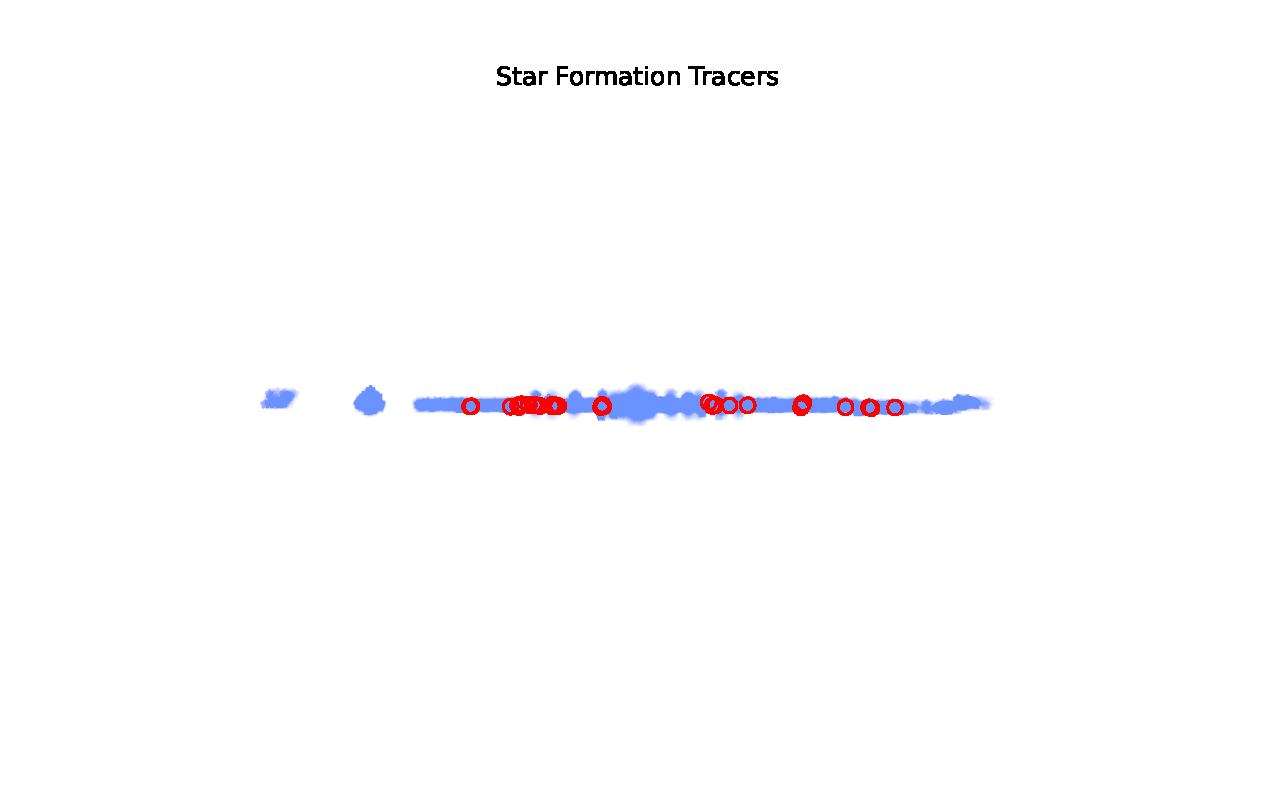
\includegraphics[width=0.8\linewidth]{Tracers_all.pdf}
    \caption{An image of the positions in longitude and latitude of YSOs (blue stars) and SFCs (red open circles) in the sky}
    \label{fig:alltracers}
\end{figure}

YSOs are stars in an early phase of their evolution, thus they are a sign of star formation. However, at low galactic latitudes, YSOs have been very difficult to detect observationally, due to dust, high stellar densities and lines of sight that pass through several star formation regions. \cite{Kuhn2021} identify $\sim$120 000 YSOs using a combination of spectral energy distribution (SED) fitting and a statistical learning method. They used photometry from the Spitzer \parencite[]{Werner_2004} and Infrared Array Camera \parencite[IRAC]{Fazio_2004} Catalogs to classify the YSOs. In addition, they looked at deeper near-infrared (NIR) photometry to distinguish them from other red objects, because YSOs are usually found in regions with high reddening. In the statistical learning model, they create training sets of YSOs from MYStIX infrared (IR) excess sources and "contaminants" which includes asymptotic giant branch stars and regions with no star formation. Then, they use a random forest classifier; this is a set of decision trees, which at each node make a "decision" based on a set of criteria, and individually make a classification. At the end of the process, the final classification is given by the majority classification of the trees. One limitation of this method is that there are still contaminants present due to the limits in observation, however, properties such as spatial distribution, photometry and optical variability suggest that most of the candidates are in fact YSOs. Finally, only 30\% of the catalog has Gaia distances, which was used to infer the distances of the other YSOs.  

The other tracer we looked at for this project was star formation complexes. \cite{RahmanMurray2010} identified 40 star formation regions from the 13 most luminous sources in the free-free emission WMAP. To identify these regions, they looked at their morphology in image mosaics using PAH emission from the Spitzer Galactic Legacy Infrared Midplane Survey Extraordinaire \parencite[GLIMPSE]{Benjamin2003} and Midcourse Space Experiment \parencite[MSX]{Price_2001} surveys. In addition, they used H\textsc{II} to determine the radial velocity of the regions, distinguish them from one another, and find their distances. One limitation was that some regions with a lot of PAH emission had no radial velocity measurements, therefore, there could be some important star formation regions not included in this analysis due to a lack of these measurements. Another limitation is that some regions have inconclusive distances from radial velocities, so instead, the "near" and "far" distances from spectroscopic absorption lines are given. 


To plot the location of the star formation tracers, we use the python package \textbf{healpy} that projects an image of a 3D sphere in 2D. We use the longitude $\phi$ and the colatitude $\theta$ to represent their positions in the sky as shown in Figure~\ref{fig:alltracers}. 

\section{Locating Star Formation Tracers on the Dust Temperature Map}


The dust temperature map shows the temperature of the dust at 9 or 17 distance slices. For this project only the map with 17 distance slices was used. In order to plot the star formation tracers at each distance in the map, we have to assign each position to one distance slice. The script does this by identifying in which distance slice range each distance is, and copying that position to a new array with the assigned distance slice (1 through 17). 

Since only 30\% of the YSOs have Gaia DR2 designations, these were the only ones plotted over the dust temperature map. Gaia does not have distances, so the distance was calculated from the parallax as shown in Equation~\ref{eq:parallaxeq}.The parallax in Gaia is in miliarcseconds so an extra step was taken to convert it into arcseconds. 9 of the 40 SFCs did not have unique distances, these were omitted for this part of the question, but later work will focus on identifying which of the 2 given distances is correct. In Figure~\ref{fig:tempmap} the positions of each is shown for two of the 17 distance slices. The images at the rest of the distance slices can be found in my GitHub repository at \url{https://github.com/molinaca/CTA200_2024/tree/main/CTA200_Project}.

\begin{equation}
    {\varpi_{i}} = 1/d  (parsecs)
    \label{eq:parallaxeq}
\end{equation}

\begin{figure}
    \centering
    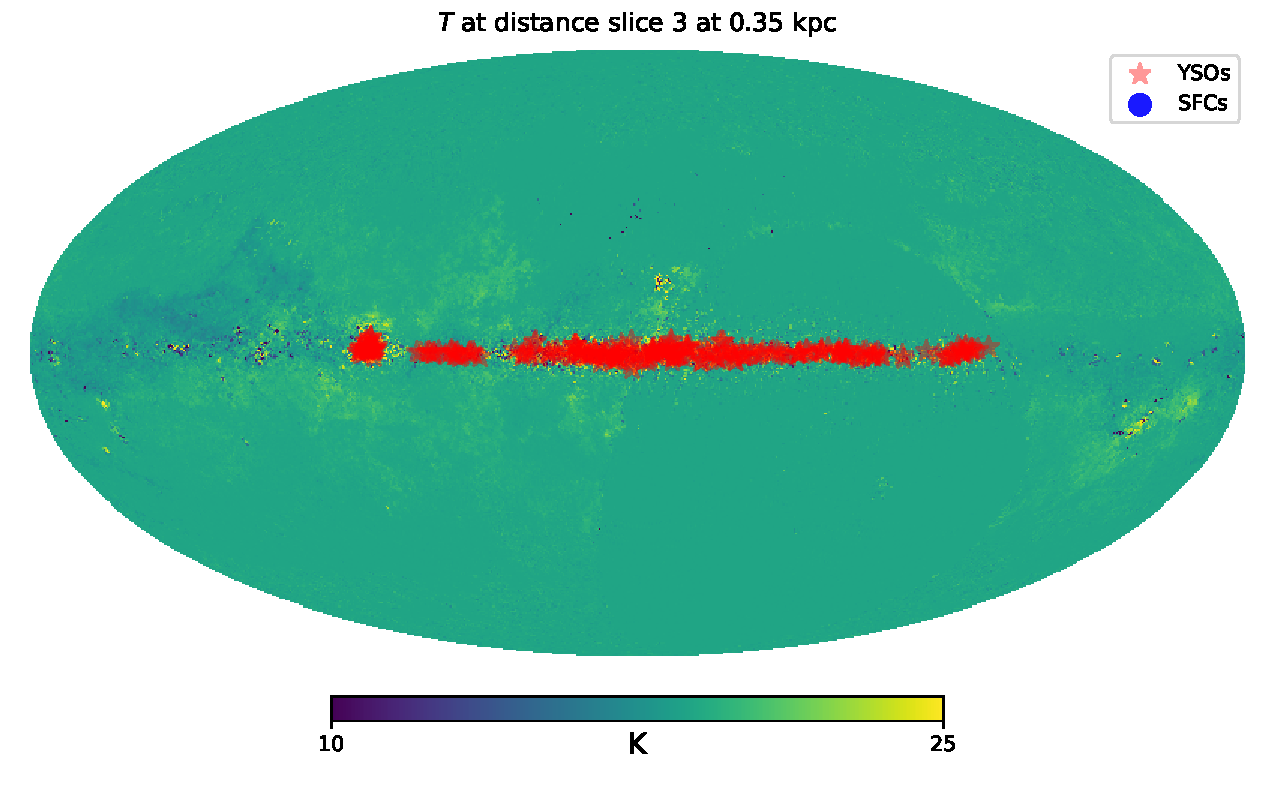
\includegraphics[width=0.75\linewidth]{tempmap_3.pdf}
    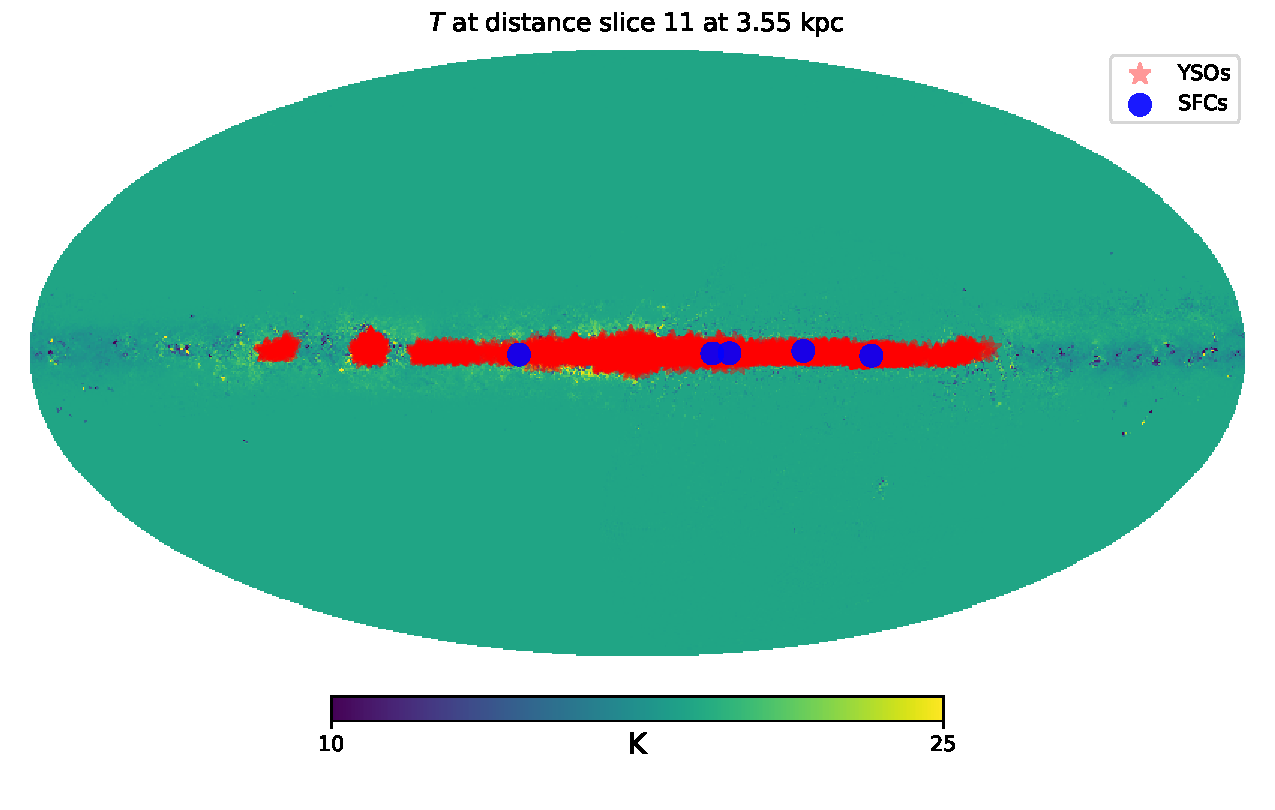
\includegraphics[width=0.75\linewidth]{tempmap_11.pdf}
    \caption{Dust temperature at distance slice 3 (top) and distance slice 11 (bottom). Overlaid is the position of the YSOs (red stars) and SFCs (blue circles) at that distance. }
    \label{fig:tempmap}
    
\end{figure}



\newpage

\printbibliography

\end{document}


%--------------------------------------------------------
%
% x.tex - end of file
%--------------------------------------------------------
